\subsection{Neural speaker recognition system}
\label{sub:speaker_recognition}
The speaker recognition system used in our experiments is based on the
framework by \cite{lukic2016speaker} and is described in Figure
\ref{fig:CNN}. The first module at the bottom is a pre-processing step that
extracts the Mel-Spectrogram from the waveform as described in section
\ref{sub:processdata}. The second module is a convolutional neural network (CNN)
that performs multi-speaker classification using the Mel-Spectrogram. The CNN is
a modified version of Alexnet~\cite{krizhevsky2012imagenet}. We warn the readers
that unlike~\cite{lukic2016speaker}, our classifier operates on 64 by 64 Mel-Spectrogram
and has slightly different number of nodes on each layer.

\begin{figure}[!ht]
    \begin{centering}
    \tikzset{ordinary/.style = {rectangle,draw,thick,rounded corners, minimum
        height = 0.5cm, minimum width=5cm, text width=5cm]}}
    \begin{tikzpicture}[node distance=0.8cm, scale=0.52, every
        node/.style={scale=0.52}]
       \node [] at (0,0) (start) {64 x 64 Mel-Spectrogram};
       \node [above=0.2cm of start] (a) {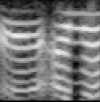
\includegraphics[width=.25\columnwidth]{figures/real_single_mel.png}};
       \node [ordinary,above=0.2cm of a] (b) {L1: convolution \hfill 3x3x32};
       \node [ordinary,above of=b] (c) {L2: max pooling \hfill 2x2};
       \node [ordinary,above of=c] (d) {L3: convolution \hfill 3x3x64};
       \node [ordinary,above of=d] (e) {L4: max pooling \hfill 2x2};
       \node [ordinary,above of=e] (f) {L5: dense \hfill 1024};
       \node [ordinary,above of=f] (g) {L6: dropout \hfill 50\%};
       \node [ordinary,above of=g] (h) {L7: dense \hfill 103};
       \node [ordinary,above of=h] (i) {L8: softmax};
       \node [above=0.2cm of i] (j) {labels};
       \draw[-] (a) -- coordinate (a) (b);
       \draw[-] (b) -- coordinate (b) (c);
       \draw[-] (c) -- coordinate (c) (d);
       \draw[-] (d) -- coordinate (d) (e);
       \draw[-] (e) -- coordinate (e) (f);
       \draw[-] (f) -- coordinate (f) (g);
       \draw[-] (g) -- coordinate (g) (h);
       \draw[-] (h) -- coordinate (h) (i);
       \draw[->] (i) -- coordinate (i) (j);
    \end{tikzpicture}
    \caption{Architecture for CNN speaker verifier.}
    \label{fig:CNN}
    \end{centering}
\end{figure}

We train our speaker classifier using 64 by 64 Mel-Spectrograms~\footnote{64 mel
bands and 64 frames, 100 ms each} from 3 speech datasets, including 100 speakers
from NIST 2004, speaker p280 from CSTR VCTK and the single speaker in Blizzard.
Our speaker classifier has a rejection path, the “other” class, trained on
environmental sounds using samples from the ESC-50 dataset. Our model achieves
approximately $85\%$ test set accuracy

\subsection{Adversarial attacks}
We define adversarial attacks on speaker recognition systems as
\textit{targeted} or \textit{untargeted}. In targeted attacks, an adversary is
interested in designing an input that makes the classification system predict a
target class chosen by the adversary. In untargeted attacks, the adversary is
interested in a confident prediction, regardless of the class being predicted as
long as it is not the "other" class.  Untargeted attacks are essentially designed
to fool the classifier into thinking a fake speech sample is real. Note that a
successful targeted attack is by definition a successful untargeted attack as
well.
